\documentclass[conference]{IEEEtran}
\IEEEoverridecommandlockouts
% The line above is only needed if you use \thanks for funding or similar notes.

\usepackage{cite}
\usepackage{amsmath,amssymb,amsfonts}
\usepackage{algorithmic}
\usepackage{graphicx}
\usepackage{textcomp}
\usepackage{xcolor}
\usepackage{tikz}

\usepackage{url}
% \usepackage[hidelinks]{hyperref}


\usepackage[
    colorlinks=true,
    linkcolor=blue,
    citecolor=blue,
    urlcolor=blue
]{hyperref}

\usetikzlibrary{arrows.meta, positioning}

\def\BibTeX{{\rm B\kern-.05em{\sc i\kern-.025em b}\kern-.08em
    T\kern-.1667em\lower.7ex\hbox{E}\kern-.125emX}}

\begin{document}
%\normalsize
\small
\title{\LARGE\bfseries From Hard Direction Decoding to Time-Dependent Low-Dimensional Neural Decoding for Hand Trajectory Estimation

%
\thanks{The neural data have been generously provided by the laboratory of Prof. Krishna Shenoy at Stanford University. The 
data are to be used exclusively for educational purposes in this course.}
}

\author{
\IEEEauthorblockN{
Yunxiang Cai, Sheng Jiang, Minghan Li, Haoqi Zhang
}
\IEEEauthorblockA{
Department of Bioengineering, Imperial College London\\
Email: \{y.cai25, sheng.jiang25, minghan.li25, haoqi.zhang25\}@imperial.ac.uk
}
}

\maketitle

\begin{abstract}
 This report evaluates two causal decoding frameworks on the BMI hand trajectory estimation task. The first employed an explicit dynamics-based framework combining SVM-based direction classification, velocity regression, and Kalman Filter to model movement evolution. The second adopted a low-dimensional decoding approach, using PCA, LDA, and kNN-based direction inference together with trajectory regression in the reduced feature space. To improve online stability, lightweight causal smoothing and trajectory blending were further incorporated. Results showed that the low-dimensional framework achieved more robust and accurate trajectory prediction than the more heavily parameterised dynamics-based approach. This suggests that, for this dataset, decoder performance depended more on matching the structure of the neural data than on increasing model complexity.
\end{abstract}


\begin{IEEEkeywords}
Brain–Machine Interface, Neural Decoding, Low-Dimensional Representation, Time-Dependent Models, Causal Decoding, Trajectory Estimation
\end{IEEEkeywords}

% Input each chapter from its own folder.
\section{Introduction}

Brain--machine interfaces (BMIs) seek to transform neural activity into useful motor outputs, making continuous trajectory decoding a central problem in prosthetic control and motor neuroscience. In this task, the objective is to estimate the planar hand trajectory of a macaque from spike trains recorded from 98 neural units during reaches to eight target directions. The decoder must remain causal, beginning prediction at 320\,ms and updating every 20\,ms using only current and past observations.

A central challenge is choosing an appropriate level of model structure. Machine learning methods for neural decoding range from simple linear models to highly expressive nonlinear approaches, and method choice remains strongly task-dependent \cite{b1}. At the same time, motor cortical population activity often evolves on low-dimensional manifolds that capture substantial task-relevant structure \cite{b2}. This suggests that improved decoding may depend not only on model complexity, but also on how well the decoder matches the latent structure of the neural data.

Motivated by this trade-off, we first explored a \textit{Hard Direction Decoder}, which performs early direction selection followed by dynamics-based trajectory estimation. We then developed a \textit{Time-Dependent PCA Decoder}, which leverages low-dimensional representations throughout the decoding process and incorporates lightweight causal stabilisation. Our results suggest that, for this dataset, robust performance is achieved more effectively through appropriate low-dimensional structure and pipeline design than through increasing model complexity alone.
\section{Methods}

This section describes the two decoding frameworks explored in this study, summarised in Fig.~\ref{fig:pipeline}. We first implemented a \textit{Hard Direction Decoder}, motivated by the widespread use of staged direction inference and state-space models in neural trajectory estimation. We then developed a \textit{Time-Dependent PCA Decoder}, which relies on compact low-dimensional representations and lightweight causal stabilisation for improved robustness.

\begin{figure}[t]
\centering
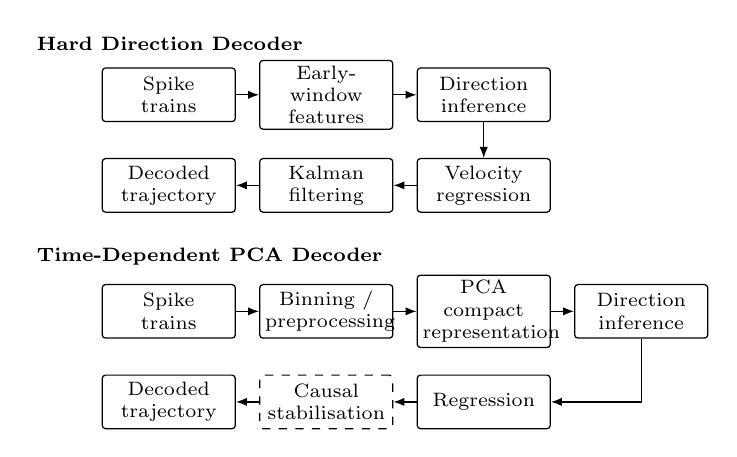
\begin{tikzpicture}[
    font=\scriptsize,
    >={Latex[length=1.4mm]},
    every path/.style={line width=0.45pt},
    box/.style={
        draw,
        rounded corners=1.2pt,
        align=center,
        minimum height=6.8mm,
        inner sep=2pt,
        text width=1.55cm
    },
    dashbox/.style={
        draw,
        dashed,
        rounded corners=1.2pt,
        align=center,
        minimum height=6.8mm,
        inner sep=2pt,
        text width=1.55cm
    },
    title/.style={
        font=\scriptsize\bfseries,
        align=left
    }
]

\begin{scope}[xshift=-0.6cm]

% ==================== Hard Direction Decoder ====================
\node[title, anchor=west] at (-1.8,0.55)
{Hard Direction Decoder};

\node[box] (a1) at (0,-0.1)    {Spike\\trains};
\node[box] (a2) at (2.0,-0.1)  {Early-window\\features};
\node[box] (a3) at (4.0,-0.1)  {Direction\\inference};

\node[box] (a4) at (0,-1.25)  {Decoded\\trajectory};
\node[box] (a5) at (2.0,-1.25) {Kalman\\filtering};
\node[box] (a6) at (4.0,-1.25) {Velocity\\regression};

\draw[->] (a1) -- (a2);
\draw[->] (a2) -- (a3);
\draw[->] (a3) -- (a6);
\draw[->] (a6) -- (a5);
\draw[->] (a5) -- (a4);

% ==================== Time-Dependent PCA Decoder ====================
\begin{scope}[yshift=0.8cm]

\node[title, anchor=west] at (-1.8,-2.95)
{Time-Dependent PCA Decoder};

\node[box] (b1) at (0,-3.65)   {Spike\\trains};
\node[box] (b2) at (2.0,-3.65) {Binning /\\preprocessing};
\node[box] (b3) at (4.0,-3.65) {PCA compact\\representation};
\node[box] (b4) at (6.0,-3.65) {Direction\\inference};

\node[box]     (b5) at (0,-4.80)   {Decoded\\trajectory};
\node[dashbox] (b6) at (2.0,-4.80) {Causal\\stabilisation};
\node[box]     (b7) at (4.0,-4.80) {Regression};

\draw[->] (b1) -- (b2);
\draw[->] (b2) -- (b3);
\draw[->] (b3) -- (b4);
\draw[->] (b4.south) |- (b7.east);
\draw[->] (b7) -- (b6);
\draw[->] (b6) -- (b5);

\end{scope}

\end{scope}
\end{tikzpicture}
\caption{Overview of the Hard Direction Decoder and the Time-Dependent PCA Decoder.}
\label{fig:pipeline}
\end{figure}

\subsection{Hard Direction Decoder}

Our initial design followed a hard direction decoding paradigm, in which movement direction is inferred early and subsequent trajectory estimation is conditioned on a single selected direction. Because motor cortical neurons are known to exhibit directional tuning during reaching \cite{b3}, the decoder first inferred movement direction from early neural activity using a supervised classifier, and then applied direction-specific continuous estimation. Among the direction-inference schemes explored during development, support vector machines (SVMs) were retained due to their empirical robustness.

Neural activity was converted into binned spike-count features, and recent spike history was used to predict two-dimensional velocity. To improve numerical stability in this regression stage, ridge regularisation was used:
\begin{equation}
\hat{W} = \arg\min_{W} \|XW - Y\|_2^2 + \lambda \|W\|_2^2,
\label{eq:ridge}
\end{equation}
where $X$ denotes neural features, $Y$ the target velocity, and $\lambda$ the regularisation coefficient. The estimated velocity was then incorporated into a state-space model. Kalman filtering was used to relate neural activity to movement kinematics \cite{b4,b5}. In its final form, the decoder employed a six-dimensional constant-acceleration state,
\begin{equation}
x_t = [p_x,\; p_y,\; v_x,\; v_y,\; a_x,\; a_y]^T,
\label{eq:state}
\end{equation}
with dynamics
\begin{equation}
x_t = A x_{t-1} + w_t, \qquad z_t = H x_t + v_t,
\label{eq:kf}
\end{equation}
where $w_t$ and $v_t$ denote process and observation noise.

To better capture trajectory variability, noise statistics were learned from training data and adjusted for early and late decoding phases. Despite these refinements, the framework remained sensitive to errors introduced in the initial direction selection stage, motivating the development of a more robust decoding strategy.

\subsection{Time-Dependent PCA Decoder}

We next adopted a low-dimensional decoding strategy based on time-dependent neural representations. This design was motivated by the observation that motor cortical activity evolves on low-dimensional manifolds that capture task-relevant structure \cite{b2}. Rather than relying on a single global model, we constructed compact representations that adapt to the available neural evidence at each time point.

Spike trains were first converted into 20\,ms bins, followed by a square-root transform and exponential moving average (EMA) smoothing to reduce noise. Features from all available causal time bins up to the current decoding time were concatenated to capture the temporal evolution of neural activity. Principal component analysis (PCA) was then applied to obtain a low-dimensional representation,
\begin{equation}
\tilde{x} = U_r^{T}(x-\mu),
\label{eq:pca}
\end{equation}
where $U_r$ contains the leading principal components.


The dimensionality $r$ was not fixed manually, but determined automatically based on a variance retention criterion. Specifically, principal components were selected such that the cumulative explained variance exceeded a predefined threshold (varKeep). 

Let $\{\lambda_i\}$ denote the eigenvalues sorted in descending order. The number of retained components $r$ is chosen as the smallest integer satisfying
\begin{equation}
\frac{\sum_{i=1}^{r} \lambda_i}{\sum_{i=1}^{D} \lambda_i} \geq \text{varKeep},
\end{equation}
where $D$ is the original feature dimension. In this work, the threshold was set to $0.85$, allowing the representation to adapt to the intrinsic structure of the data while avoiding unnecessary high-dimensional noise.


In this reduced space, linear discriminant analysis (LDA) was used to enhance separation between movement directions, and direction inference was performed using distance-weighted $k$-nearest neighbours. This combination provided a compact, discriminative, and locally adaptive representation of neural activity.

Trajectory-related quantities were then estimated using direction-conditioned regression models in the reduced feature space. Compared with a single global mapping, this formulation enabled smoother and more stable neural-to-kinematic predictions while maintaining causality.

\subsection{Lightweight Causal Stabilisation}

Although the low-dimensional decoder was more robust, early-stage predictions could still exhibit instability due to directional uncertainty. We therefore introduced lightweight causal stabilisation mechanisms.

First, instead of relying on a single hard direction estimate, predictions from multiple candidate directions were softly combined:
\begin{equation}
\hat{y}=\sum_{m=1}^{M} w_m \hat{y}_m, \qquad \sum_{m=1}^{M} w_m = 1,
\label{eq:ensemble}
\end{equation}
which reduced sensitivity to early misclassification. Second, predictions were blended with direction-specific mean trajectories, with the influence of the mean decaying over time. 
%这里删掉了
%Third, displacement clipping was applied to suppress implausible jumps. %Finally, lightweight causal smoothing was used to reduce high-frequency jitter.

All operations were strictly causal and relied only on past and current observations. These mechanisms did not replace the core decoder, but improved stability while preserving a compact and interpretable structure.
\section{Results}

We evaluated decoding performance using the root mean squared error (RMSE) of the reconstructed trajectories, together with runtime and the competition score. Table~\ref{tab:hard_decoder} summarises representative results from the Hard Direction Decoder, while Table~\ref{tab:pca_decoder} reports the performance of the proposed Time-Dependent PCA Decoder.

\begin{table}[htbp]
\centering
\caption{Performance of the Hard Direction Decoder (representative variants).}
\label{tab:hard_decoder}
\begin{tabular}{lccc}
\hline
Method & RMSE & Time (s) & Score \\
\hline
Template + Ridge + Integration & 21.82 & 1.57 & 19.79 \\
Template + PCA + Ridge + Kalman & 21.09 & 1.85 & 19.17 \\
SVM + Ridge + Kalman & 22.28 & 3.59 & 20.41 \\
SVM + Ridge + learned CA-KF & 22.09 & 2.61 & 20.14 \\
\hline
\end{tabular}
\end{table}

Within the Hard Direction Decoder, improvements such as PCA-based denoising, alternative classifiers (e.g., SVM), and refined Kalman filtering resulted in only modest performance gains, with RMSE remaining around 21--23.

\begin{table}[htbp]
\centering
\caption{Performance of the Time-Dependent PCA Decoder.}
\label{tab:pca_decoder}
\begin{tabular}{lccc}
\hline
Method & RMSE & Time (s) & Score \\
\hline
Baseline time-dependent model & 8.03 & 3.44 & 7.57 \\
+ soft direction blending & 7.83 & 3.42 & 7.38 \\
Final model (tuned PCA + smoothing) & \textbf{7.50} & 3.17 & \textbf{7.07} \\
\hline
\end{tabular}
\end{table}

In contrast, the proposed Time-Dependent PCA Decoder achieved a substantially lower RMSE of approximately 7.5, representing a significant improvement over the Hard Direction Decoder. This indicates that redesigning the decoding pipeline is more effective than refining individual components within a fixed structure.\\

The performance gain can be attributed to three main factors. First, PCA-based low-dimensional representations provide a compact and noise-robust description of neural activity. Second, direction inference in this reduced space improves reliability compared to early hard decisions. Third, soft blending of multiple candidate directions and lightweight causal stabilisation reduce sensitivity to early decoding errors and improve temporal consistency.


\begin{figure}[htbp]
\centerline{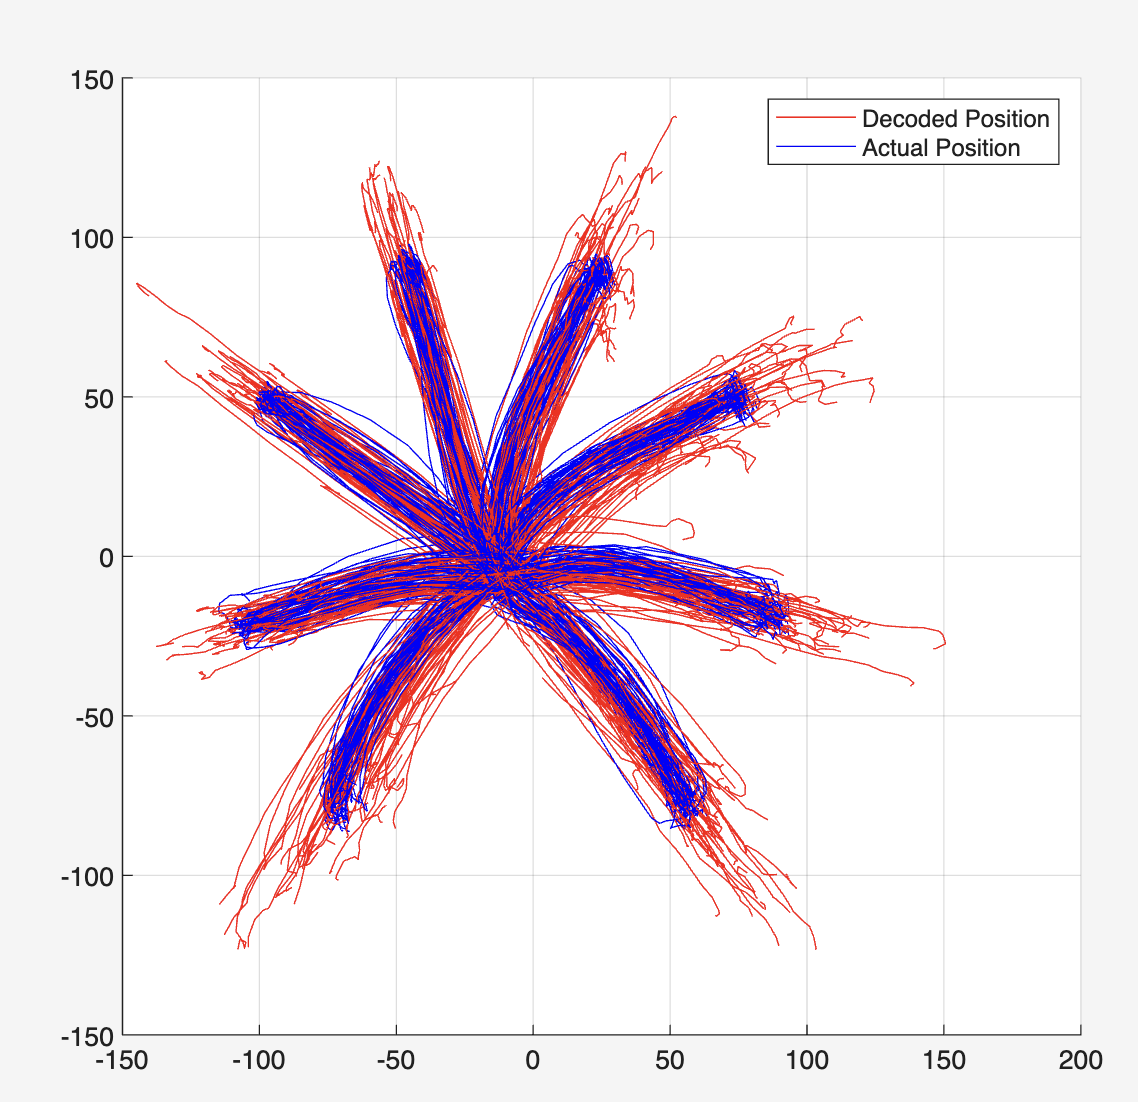
\includegraphics[width=0.85\columnwidth]{results/hand-position-estimation-using-hard-direction-decoder-v1.png}}
\caption{Decoded trajectories (red) versus ground truth (blue) using the Hard Direction Decoder. The decoded paths capture the general reaching directions, but show larger deviations and greater trajectory spread, reflecting sensitivity to early hard direction selection and accumulated estimation error.}
\label{fig:hard_trajectory}
\end{figure}

\begin{figure}[htbp]
\centerline{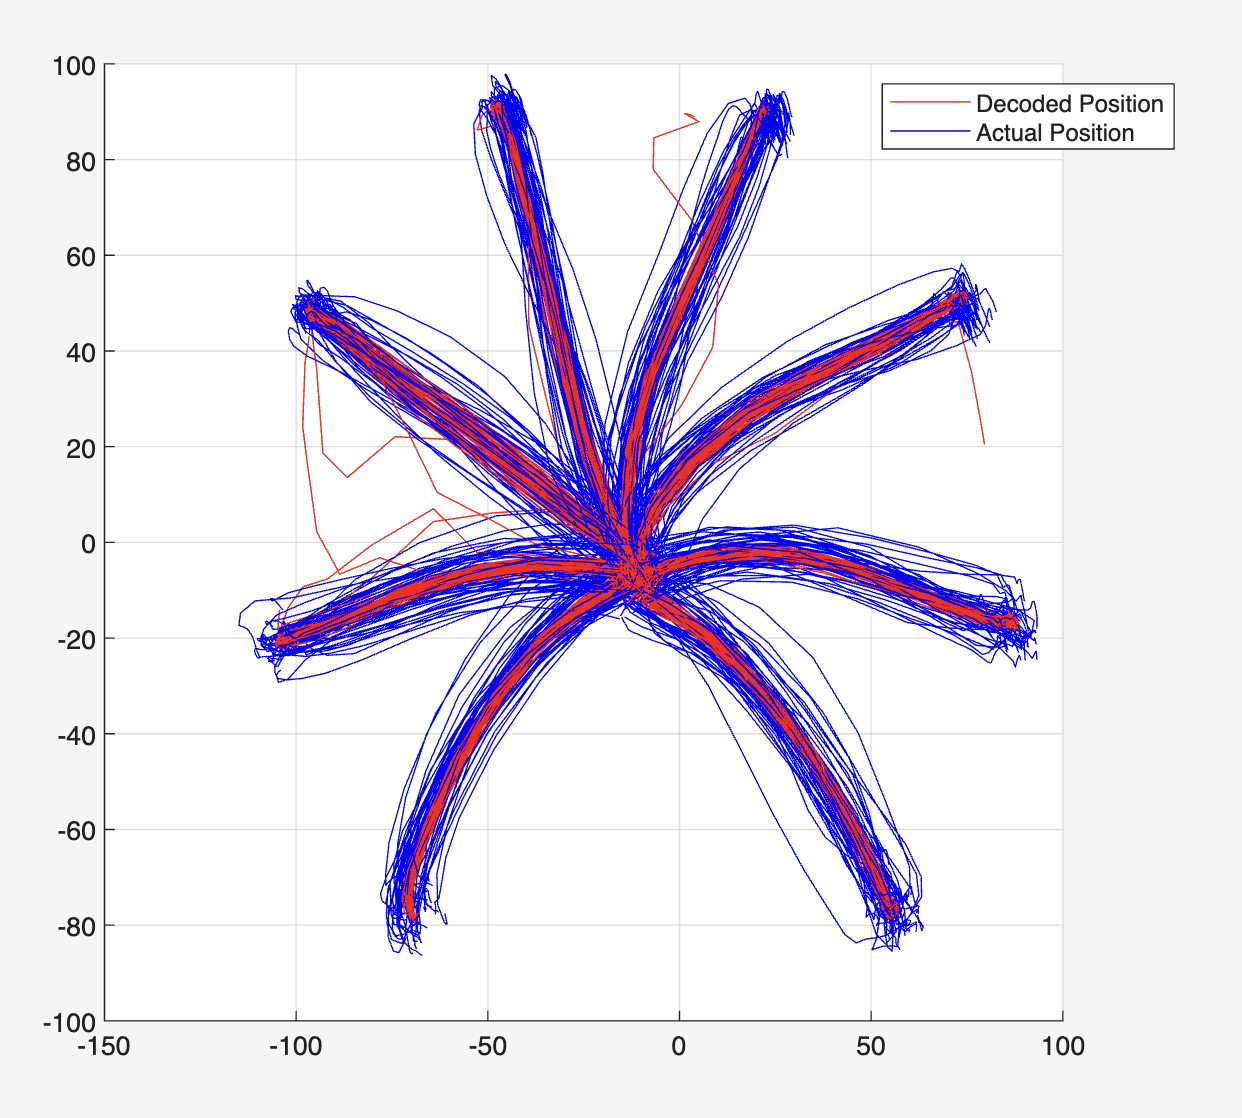
\includegraphics[width=0.85\columnwidth]{results/hand-position-estimation-using-time-dependent-pca-decoder-v5.png}}
\caption{Decoded trajectories (red) versus ground truth (blue) using the Time-Dependent PCA Decoder. Compared with the Hard Direction Decoder, the decoded trajectories are more tightly aligned with the true movements and show smoother behaviour across reaching directions.}
\label{fig:pca_trajectory}
\end{figure}

Figure~\ref{fig:hard_trajectory} shows that the Hard Direction Decoder captures the overall radial structure of the reaching task, but produces visibly larger deviations from the true trajectories. In contrast, Fig.~\ref{fig:pca_trajectory} shows that the Time-Dependent PCA Decoder generates trajectories that are more tightly aligned with the ground truth, consistent with its lower RMSE.

Figure~\ref{fig:pca_trajectory} illustrates representative decoded trajectories. The proposed method closely follows the ground truth across all reaching directions, while maintaining smooth and consistent trajectories over time.


Overall, these results demonstrate that appropriate use of low-dimensional structure and pipeline design leads to substantial improvements in decoding accuracy, while remaining fully causal and computationally efficient.

\begin{figure}[htbp]
\centerline{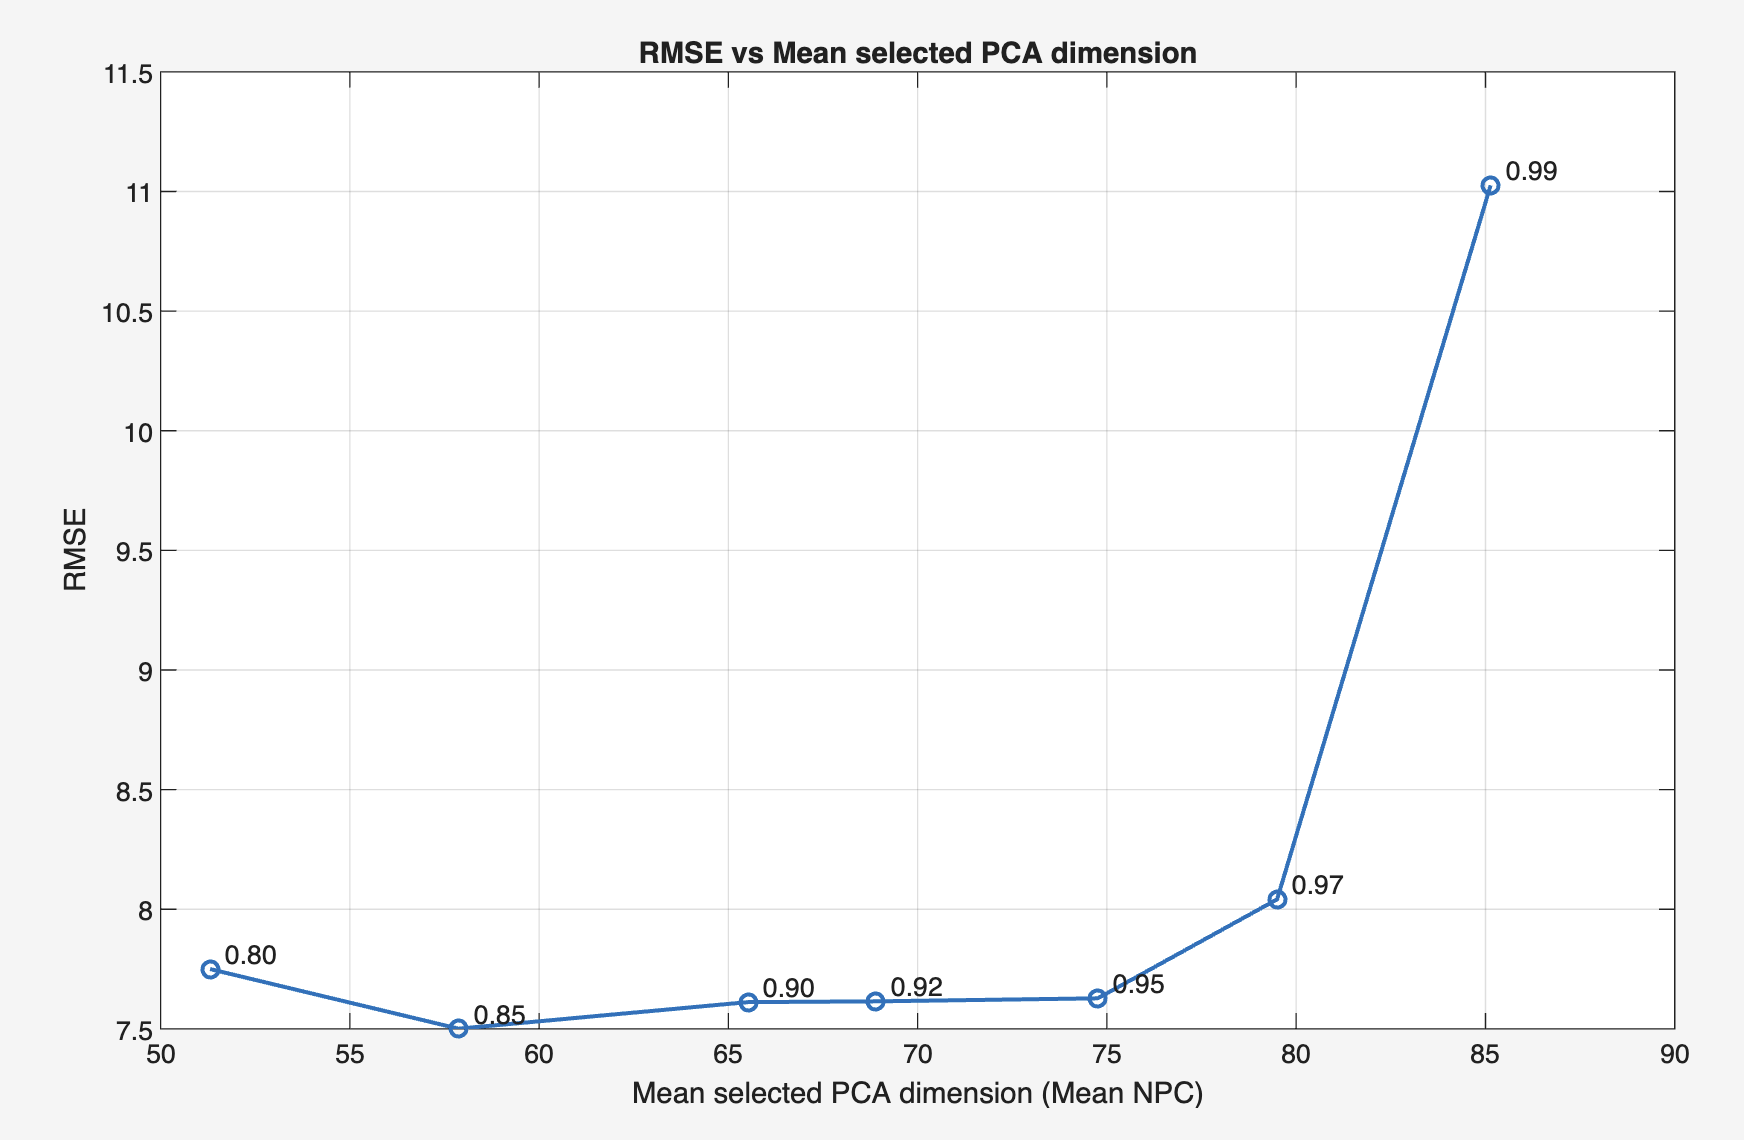
\includegraphics[width=0.95\columnwidth]{results/RMSE-vs-Mean-Selected-PCA-Dimension-v5.png}}
\caption{RMSE as a function of the mean number of selected PCA dimensions. Each point corresponds to a different variance retention threshold. An intermediate dimensionality achieves the best performance, while too few or too many components lead to increased error.}
\label{fig:pca_dimension}
\end{figure}

We further analysed the effect of PCA dimensionality on decoding performance (Fig.~\ref{fig:pca_dimension}). The results show a non-monotonic relationship between the number of retained principal components and RMSE.

Best performance is achieved at an intermediate dimensionality, corresponding to a variance retention of approximately 0.85. When too few components are retained, important task-relevant information is lost. In contrast, retaining too many components introduces noise and degrades performance.

This result highlights the importance of balancing information preservation and noise suppression when constructing low-dimensional neural representations.
\section{Discussion}

The results of this study highlight that decoding performance is influenced more by the overall pipeline structure than by the choice of individual components. While the Hard Direction Decoder incorporated increasingly sophisticated elements, including SVM-based classification and Kalman filtering, these refinements resulted in only marginal improvements. This suggests that improving individual modules within a fixed architecture is insufficient when the underlying information flow is suboptimal.

A key limitation of the Hard Direction Decoder lies in its reliance on early hard direction selection. Errors made at this stage propagate through subsequent velocity estimation and state-space filtering, leading to persistent trajectory deviations. In contrast, the proposed Time-Dependent PCA Decoder mitigates this issue by delaying commitment to a single direction and allowing multiple candidate directions to contribute through soft combination. This reduces sensitivity to early uncertainty and improves robustness in the causal decoding setting.

Another important factor is the use of time-dependent models. By constructing separate representations for different time points, the decoder adapts to the amount of available neural information as the movement unfolds. Early predictions rely on compact, noise-robust features, while later predictions benefit from richer temporal context. This contrasts with a static model, which must balance these competing requirements globally.

The use of PCA further supports this design by providing a low-dimensional representation that captures task-relevant neural structure while suppressing noise. Importantly, the dimensionality is selected automatically based on a variance retention criterion, avoiding manual tuning and enabling the representation to adapt to the intrinsic structure of the data. As shown in the results, decoding performance depends critically on this balance: overly aggressive dimensionality reduction leads to information loss, whereas retaining too many components introduces noise.

Finally, the proposed approach achieves these improvements without relying on complex state-space models. Instead, lightweight causal smoothing and feature-based temporal integration provide sufficient stability for accurate trajectory reconstruction. This demonstrates that, for this task, appropriate use of low-dimensional structure and pipeline design can outperform more complex dynamic models while remaining computationally efficient and fully causal.

Overall, these findings suggest that effective neural decoding depends not only on model complexity, but more importantly on how information is structured, represented, and propagated through the decoding pipeline.
\section{Conclusion}

In this work, we investigated neural trajectory decoding under a strictly causal setting and compared two decoding strategies: a Hard Direction Decoder and a Time-Dependent PCA Decoder. While the former relies on early direction classification followed by model-based trajectory estimation, the latter adopts a low-dimensional, time-dependent representation combined with lightweight stabilisation.

Our results show that substantial performance improvements are achieved not by increasing model complexity, but by redesigning the decoding pipeline. In particular, the use of time-dependent representations, PCA-based dimensionality reduction, and soft direction combination significantly improves robustness and reduces error propagation, leading to a marked reduction in RMSE.

These findings suggest that effective neural decoding depends critically on how information is represented and integrated over time. Future work may explore extending this framework to more complex movement tasks or incorporating adaptive representations that further capture nonlinear neural dynamics.


The implementation of the proposed methods is available at: \url{https://github.com/shengj1ang/DanceMonkey}.

\section*{Acknowledgment}
We would like to express their sincere gratitude to Dr.\ Clopath Claudia, and all the GTAs for their valuable guidance, feedback, and support throughout this project.

\section*{Attributions}

All team members contributed actively and collaboratively throughout the project, from method development to result analysis and report preparation.

Yunxiang Cai contributed the optimisation and final refinement of the Time-Dependent PCA Decoder. This included improving the overall decoding pipeline, tuning key components of the final low-dimensional framework, and consolidating the version used for the final experiments and report. 

Sheng Jiang led to the initial development of the Time-Dependent PCA Decoder and was primarily responsible for data visualisation and figure generation. This included preparing plots and graphical materials used to support the analysis, comparison of decoder behaviour, and presentation of results in the report. 

Minghan Li developed the Hard Direction Decoder and explored multiple variants of this framework during the earlier stage of the project. This work involved investigating different formulations of direction-based decoding and assessing their performance as part of the team’s iterative model development process. 

Haoqi Zhang contributed to the development of the Hard Direction Decoder and participated in the initial structuring and drafting of the report. This included helping organise the narrative of the study, shaping the methodological presentation, and contributing to the written explanation of the project’s progression.

Besides these main duties, each member participated in group discussions, experimental design, interpretation of outcomes and final report revision. This project was done on a team basis where the final submission represented collective discussion and collective refinement at every stage of the work.

\section*{AI Use Statement}
Artificial intelligence tools were used in a supportive capacity during this project.

AI tools were utilized in report writing to help in language polishing, grammar correction, sentence restructuring, refining academic phrasing, and better section organization. The tools were also used to assist when making technical descriptions, captions of figures and interpretation of results simpler and shorter.

In literature research, AI was used as a source that could assist in finding and summarising important pieces of literature related to neural decoding, Kalman filtering, low-dimensional neural representation and estimation of trajectories. It helped the group to know why the first explicit dynamics based framework did not show much improvement and think about other low-dimensional decoding approach. Selection, verification, and interpretation of the literature, as well as the choice to change the modeling direction, were performed by the team.

AI tools were used in order to offer directions on debugging, clarify problems with clearer comments, and enhance the readability or organization of code. They were additionally used in assisting to discuss some of the potential causes of underperforming model variants including feature construction, direction inference stability and interaction of decoding stages.

The detailed decoding algorithms, submitted results and the final scientific conclusion are not generated using AI tools. The main intellectual work, such as formulating the problem, model design and implementation, parameters choosing, experimental assessment, interpreting results, and critically discussing them has been carried out by the team.


% Use BibTeX for the reference list.
\bibliographystyle{IEEEtran}
\bibliography{references}

\end{document}